% Created by tikzDevice version 0.10.1 on 2016-05-08 18:26:22
% !TEX encoding = UTF-8 Unicode
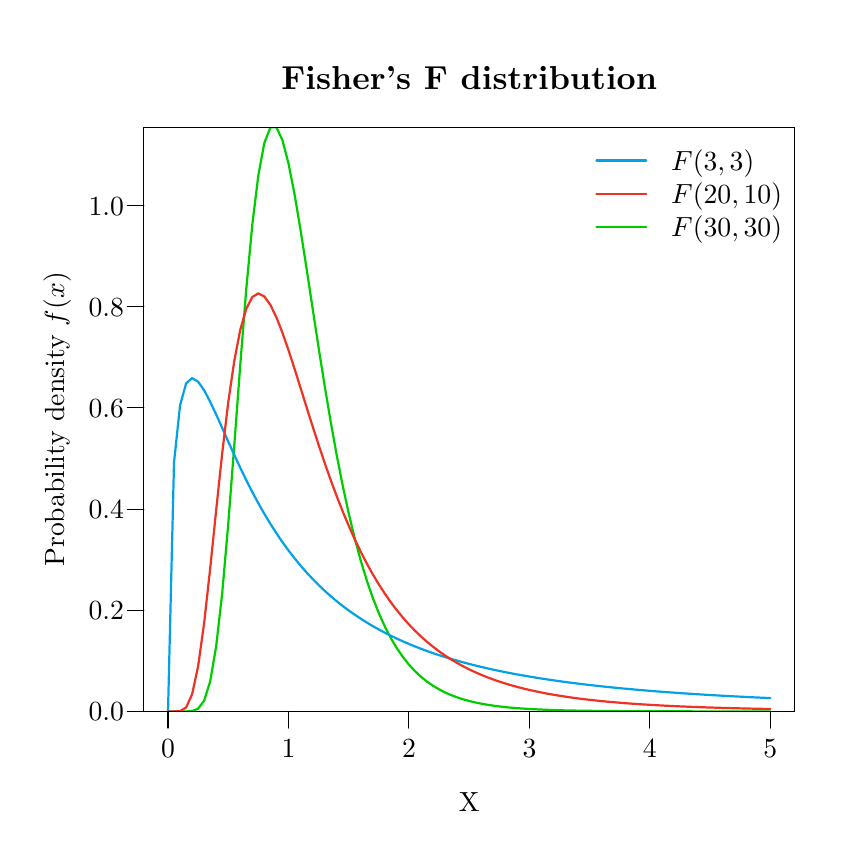
\begin{tikzpicture}[x=1pt,y=1pt]
\definecolor{fillColor}{RGB}{255,255,255}
\path[use as bounding box,fill=fillColor,fill opacity=0.00] (0,0) rectangle (289.08,289.08);
\begin{scope}
\path[clip] ( 42.00, 42.00) rectangle (277.08,253.08);
\definecolor{drawColor}{RGB}{0,205,0}

\path[draw=drawColor,line width= 0.8pt,line join=round,line cap=round] ( 50.71, 42.00) --
	( 52.88, 42.00) --
	( 55.06, 42.00) --
	( 57.24, 42.01) --
	( 59.41, 42.15) --
	( 61.59, 42.98) --
	( 63.77, 45.88) --
	( 65.94, 52.83) --
	( 68.12, 65.59) --
	( 70.30, 84.81) --
	( 72.47,109.69) --
	( 74.65,138.11) --
	( 76.83,167.37) --
	( 79.00,194.73) --
	( 81.18,218.02) --
	( 83.36,235.81) --
	( 85.53,247.47) --
	( 87.71,253.04) --
	( 89.89,253.08) --
	( 92.06,248.42) --
	( 94.24,240.04) --
	( 96.42,228.94) --
	( 98.59,216.01) --
	(100.77,202.06) --
	(102.95,187.72) --
	(105.12,173.50) --
	(107.30,159.77) --
	(109.48,146.78) --
	(111.65,134.71) --
	(113.83,123.63) --
	(116.01,113.57) --
	(118.18,104.53) --
	(120.36, 96.47) --
	(122.54, 89.32) --
	(124.71, 83.02) --
	(126.89, 77.50) --
	(129.07, 72.67) --
	(131.24, 68.47) --
	(133.42, 64.82) --
	(135.60, 61.66) --
	(137.77, 58.92) --
	(139.95, 56.56) --
	(142.13, 54.53) --
	(144.30, 52.78) --
	(146.48, 51.27) --
	(148.66, 49.97) --
	(150.83, 48.86) --
	(153.01, 47.91) --
	(155.19, 47.08) --
	(157.36, 46.38) --
	(159.54, 45.77) --
	(161.72, 45.25) --
	(163.89, 44.81) --
	(166.07, 44.42) --
	(168.25, 44.09) --
	(170.42, 43.81) --
	(172.60, 43.56) --
	(174.78, 43.35) --
	(176.95, 43.17) --
	(179.13, 43.02) --
	(181.31, 42.88) --
	(183.48, 42.77) --
	(185.66, 42.67) --
	(187.84, 42.58) --
	(190.01, 42.50) --
	(192.19, 42.44) --
	(194.37, 42.38) --
	(196.54, 42.33) --
	(198.72, 42.29) --
	(200.90, 42.25) --
	(203.07, 42.22) --
	(205.25, 42.20) --
	(207.43, 42.17) --
	(209.60, 42.15) --
	(211.78, 42.13) --
	(213.96, 42.12) --
	(216.13, 42.10) --
	(218.31, 42.09) --
	(220.49, 42.08) --
	(222.66, 42.07) --
	(224.84, 42.06) --
	(227.02, 42.05) --
	(229.19, 42.05) --
	(231.37, 42.04) --
	(233.55, 42.04) --
	(235.72, 42.03) --
	(237.90, 42.03) --
	(240.08, 42.03) --
	(242.25, 42.02) --
	(244.43, 42.02) --
	(246.61, 42.02) --
	(248.78, 42.02) --
	(250.96, 42.01) --
	(253.14, 42.01) --
	(255.31, 42.01) --
	(257.49, 42.01) --
	(259.67, 42.01) --
	(261.84, 42.01) --
	(264.02, 42.01) --
	(266.20, 42.01) --
	(268.37, 42.01);
\end{scope}
\begin{scope}
\path[clip] (  0.00,  0.00) rectangle (289.08,289.08);
\definecolor{drawColor}{RGB}{0,0,0}

\path[draw=drawColor,line width= 0.4pt,line join=round,line cap=round] ( 50.71, 42.00) -- (268.37, 42.00);

\path[draw=drawColor,line width= 0.4pt,line join=round,line cap=round] ( 50.71, 42.00) -- ( 50.71, 36.00);

\path[draw=drawColor,line width= 0.4pt,line join=round,line cap=round] ( 94.24, 42.00) -- ( 94.24, 36.00);

\path[draw=drawColor,line width= 0.4pt,line join=round,line cap=round] (137.77, 42.00) -- (137.77, 36.00);

\path[draw=drawColor,line width= 0.4pt,line join=round,line cap=round] (181.31, 42.00) -- (181.31, 36.00);

\path[draw=drawColor,line width= 0.4pt,line join=round,line cap=round] (224.84, 42.00) -- (224.84, 36.00);

\path[draw=drawColor,line width= 0.4pt,line join=round,line cap=round] (268.37, 42.00) -- (268.37, 36.00);

\node[text=drawColor,anchor=base,inner sep=0pt, outer sep=0pt, scale=  1.00] at ( 50.71, 25.20) {0};

\node[text=drawColor,anchor=base,inner sep=0pt, outer sep=0pt, scale=  1.00] at ( 94.24, 25.20) {1};

\node[text=drawColor,anchor=base,inner sep=0pt, outer sep=0pt, scale=  1.00] at (137.77, 25.20) {2};

\node[text=drawColor,anchor=base,inner sep=0pt, outer sep=0pt, scale=  1.00] at (181.31, 25.20) {3};

\node[text=drawColor,anchor=base,inner sep=0pt, outer sep=0pt, scale=  1.00] at (224.84, 25.20) {4};

\node[text=drawColor,anchor=base,inner sep=0pt, outer sep=0pt, scale=  1.00] at (268.37, 25.20) {5};

\path[draw=drawColor,line width= 0.4pt,line join=round,line cap=round] ( 42.00, 42.00) -- ( 42.00,224.78);

\path[draw=drawColor,line width= 0.4pt,line join=round,line cap=round] ( 42.00, 42.00) -- ( 36.00, 42.00);

\path[draw=drawColor,line width= 0.4pt,line join=round,line cap=round] ( 42.00, 78.56) -- ( 36.00, 78.56);

\path[draw=drawColor,line width= 0.4pt,line join=round,line cap=round] ( 42.00,115.11) -- ( 36.00,115.11);

\path[draw=drawColor,line width= 0.4pt,line join=round,line cap=round] ( 42.00,151.67) -- ( 36.00,151.67);

\path[draw=drawColor,line width= 0.4pt,line join=round,line cap=round] ( 42.00,188.23) -- ( 36.00,188.23);

\path[draw=drawColor,line width= 0.4pt,line join=round,line cap=round] ( 42.00,224.78) -- ( 36.00,224.78);

\node[text=drawColor,anchor=base east,inner sep=0pt, outer sep=0pt, scale=  1.00] at ( 34.80, 38.56) {0.0};

\node[text=drawColor,anchor=base east,inner sep=0pt, outer sep=0pt, scale=  1.00] at ( 34.80, 75.11) {0.2};

\node[text=drawColor,anchor=base east,inner sep=0pt, outer sep=0pt, scale=  1.00] at ( 34.80,111.67) {0.4};

\node[text=drawColor,anchor=base east,inner sep=0pt, outer sep=0pt, scale=  1.00] at ( 34.80,148.23) {0.6};

\node[text=drawColor,anchor=base east,inner sep=0pt, outer sep=0pt, scale=  1.00] at ( 34.80,184.78) {0.8};

\node[text=drawColor,anchor=base east,inner sep=0pt, outer sep=0pt, scale=  1.00] at ( 34.80,221.34) {1.0};

\path[draw=drawColor,line width= 0.4pt,line join=round,line cap=round] ( 42.00, 42.00) --
	(277.08, 42.00) --
	(277.08,253.08) --
	( 42.00,253.08) --
	( 42.00, 42.00);
\end{scope}
\begin{scope}
\path[clip] (  0.00,  0.00) rectangle (289.08,289.08);
\definecolor{drawColor}{RGB}{0,0,0}

\node[text=drawColor,anchor=base,inner sep=0pt, outer sep=0pt, scale=  1.20] at (159.54,266.89) {\bfseries Fisher's F distribution};

\node[text=drawColor,anchor=base,inner sep=0pt, outer sep=0pt, scale=  1.00] at (159.54,  6.00) {X};

\node[text=drawColor,rotate= 90.00,anchor=base,inner sep=0pt, outer sep=0pt, scale=  1.00] at ( 13.20,147.54) {Probability density $f(x)$};
\end{scope}
\begin{scope}
\path[clip] ( 42.00, 42.00) rectangle (277.08,253.08);
\definecolor{drawColor}{RGB}{5,161,230}

\path[draw=drawColor,line width= 0.8pt,line join=round,line cap=round] ( 50.71, 42.00) --
	( 52.88,131.91) --
	( 55.06,152.59) --
	( 57.24,160.53) --
	( 59.41,162.46) --
	( 61.59,161.16) --
	( 63.77,158.04) --
	( 65.94,153.92) --
	( 68.12,149.28) --
	( 70.30,144.42) --
	( 72.47,139.52) --
	( 74.65,134.70) --
	( 76.83,130.02) --
	( 79.00,125.54) --
	( 81.18,121.26) --
	( 83.36,117.21) --
	( 85.53,113.38) --
	( 87.71,109.78) --
	( 89.89,106.38) --
	( 92.06,103.18) --
	( 94.24,100.18) --
	( 96.42, 97.36) --
	( 98.59, 94.71) --
	(100.77, 92.22) --
	(102.95, 89.89) --
	(105.12, 87.69) --
	(107.30, 85.62) --
	(109.48, 83.67) --
	(111.65, 81.84) --
	(113.83, 80.11) --
	(116.01, 78.48) --
	(118.18, 76.95) --
	(120.36, 75.50) --
	(122.54, 74.13) --
	(124.71, 72.83) --
	(126.89, 71.61) --
	(129.07, 70.45) --
	(131.24, 69.35) --
	(133.42, 68.31) --
	(135.60, 67.32) --
	(137.77, 66.38) --
	(139.95, 65.49) --
	(142.13, 64.64) --
	(144.30, 63.84) --
	(146.48, 63.07) --
	(148.66, 62.34) --
	(150.83, 61.64) --
	(153.01, 60.98) --
	(155.19, 60.35) --
	(157.36, 59.74) --
	(159.54, 59.17) --
	(161.72, 58.61) --
	(163.89, 58.09) --
	(166.07, 57.58) --
	(168.25, 57.10) --
	(170.42, 56.64) --
	(172.60, 56.19) --
	(174.78, 55.77) --
	(176.95, 55.36) --
	(179.13, 54.97) --
	(181.31, 54.60) --
	(183.48, 54.24) --
	(185.66, 53.89) --
	(187.84, 53.56) --
	(190.01, 53.24) --
	(192.19, 52.93) --
	(194.37, 52.63) --
	(196.54, 52.35) --
	(198.72, 52.08) --
	(200.90, 51.81) --
	(203.07, 51.56) --
	(205.25, 51.31) --
	(207.43, 51.07) --
	(209.60, 50.84) --
	(211.78, 50.62) --
	(213.96, 50.41) --
	(216.13, 50.20) --
	(218.31, 50.01) --
	(220.49, 49.81) --
	(222.66, 49.63) --
	(224.84, 49.45) --
	(227.02, 49.27) --
	(229.19, 49.10) --
	(231.37, 48.94) --
	(233.55, 48.78) --
	(235.72, 48.63) --
	(237.90, 48.48) --
	(240.08, 48.34) --
	(242.25, 48.20) --
	(244.43, 48.07) --
	(246.61, 47.93) --
	(248.78, 47.81) --
	(250.96, 47.68) --
	(253.14, 47.56) --
	(255.31, 47.45) --
	(257.49, 47.34) --
	(259.67, 47.23) --
	(261.84, 47.12) --
	(264.02, 47.02) --
	(266.20, 46.92) --
	(268.37, 46.82);
\definecolor{drawColor}{RGB}{238,50,36}

\path[draw=drawColor,line width= 0.8pt,line join=round,line cap=round] ( 50.71, 42.00) --
	( 52.88, 42.00) --
	( 55.06, 42.12) --
	( 57.24, 43.41) --
	( 59.41, 48.17) --
	( 61.59, 58.32) --
	( 63.77, 73.99) --
	( 65.94, 93.59) --
	( 68.12,114.80) --
	( 70.30,135.39) --
	( 72.47,153.67) --
	( 74.65,168.66) --
	( 76.83,179.94) --
	( 79.00,187.54) --
	( 81.18,191.76) --
	( 83.36,193.05) --
	( 85.53,191.93) --
	( 87.71,188.89) --
	( 89.89,184.39) --
	( 92.06,178.84) --
	( 94.24,172.57) --
	( 96.42,165.87) --
	( 98.59,158.94) --
	(100.77,151.96) --
	(102.95,145.07) --
	(105.12,138.35) --
	(107.30,131.87) --
	(109.48,125.69) --
	(111.65,119.82) --
	(113.83,114.28) --
	(116.01,109.08) --
	(118.18,104.22) --
	(120.36, 99.68) --
	(122.54, 95.46) --
	(124.71, 91.54) --
	(126.89, 87.90) --
	(129.07, 84.54) --
	(131.24, 81.42) --
	(133.42, 78.55) --
	(135.60, 75.89) --
	(137.77, 73.43) --
	(139.95, 71.17) --
	(142.13, 69.08) --
	(144.30, 67.15) --
	(146.48, 65.37) --
	(148.66, 63.72) --
	(150.83, 62.20) --
	(153.01, 60.80) --
	(155.19, 59.50) --
	(157.36, 58.31) --
	(159.54, 57.20) --
	(161.72, 56.18) --
	(163.89, 55.23) --
	(166.07, 54.35) --
	(168.25, 53.54) --
	(170.42, 52.79) --
	(172.60, 52.09) --
	(174.78, 51.44) --
	(176.95, 50.84) --
	(179.13, 50.29) --
	(181.31, 49.77) --
	(183.48, 49.29) --
	(185.66, 48.84) --
	(187.84, 48.42) --
	(190.01, 48.03) --
	(192.19, 47.67) --
	(194.37, 47.33) --
	(196.54, 47.02) --
	(198.72, 46.73) --
	(200.90, 46.45) --
	(203.07, 46.20) --
	(205.25, 45.96) --
	(207.43, 45.73) --
	(209.60, 45.52) --
	(211.78, 45.33) --
	(213.96, 45.15) --
	(216.13, 44.97) --
	(218.31, 44.81) --
	(220.49, 44.66) --
	(222.66, 44.52) --
	(224.84, 44.39) --
	(227.02, 44.26) --
	(229.19, 44.14) --
	(231.37, 44.03) --
	(233.55, 43.93) --
	(235.72, 43.83) --
	(237.90, 43.74) --
	(240.08, 43.65) --
	(242.25, 43.57) --
	(244.43, 43.49) --
	(246.61, 43.42) --
	(248.78, 43.35) --
	(250.96, 43.28) --
	(253.14, 43.22) --
	(255.31, 43.16) --
	(257.49, 43.11) --
	(259.67, 43.06) --
	(261.84, 43.01) --
	(264.02, 42.96) --
	(266.20, 42.92) --
	(268.37, 42.88);
\definecolor{drawColor}{RGB}{5,161,230}

\path[draw=drawColor,line width= 0.8pt,line join=round,line cap=round] (205.54,241.08) -- (223.54,241.08);
\definecolor{drawColor}{RGB}{238,50,36}

\path[draw=drawColor,line width= 0.8pt,line join=round,line cap=round] (205.54,229.08) -- (223.54,229.08);
\definecolor{drawColor}{RGB}{0,205,0}

\path[draw=drawColor,line width= 0.8pt,line join=round,line cap=round] (205.54,217.08) -- (223.54,217.08);
\definecolor{drawColor}{RGB}{0,0,0}

\node[text=drawColor,anchor=base west,inner sep=0pt, outer sep=0pt, scale=  1.00] at (232.54,237.64) {$F(3,3)$};

\node[text=drawColor,anchor=base west,inner sep=0pt, outer sep=0pt, scale=  1.00] at (232.54,225.64) {$F(20,10)$};

\node[text=drawColor,anchor=base west,inner sep=0pt, outer sep=0pt, scale=  1.00] at (232.54,213.64) {$F(30,30)$};
\end{scope}
\begin{scope}
\path[clip] (  0.00,  0.00) rectangle (289.08,289.08);
\definecolor{drawColor}{RGB}{0,0,0}

\path[draw=drawColor,line width= 0.4pt,line join=round,line cap=round] ( 42.00, 42.00) --
	(277.08, 42.00) --
	(277.08,253.08) --
	( 42.00,253.08) --
	( 42.00, 42.00);
\end{scope}
\end{tikzpicture}
